\subsection{$\pi^0$-rich sidebands}
\label{sec:sideband:pi0}
Measuring events with final-state $\pi^0 \rightarrow \gamma\gamma$ plays an important role for this analysis as they provide a high-statistics sample of low-energy (50-300 MeV) EM showers with which to validate shower reconstruction and energy calibrations, and a necessary data-driven constraint of $\pi^0$ backgrounds to the analysis.

\subsubsection{EM shower validations with {$\pi^0 \rightarrow \gamma\gamma$ events}}

The validation of EM shower reconstruction is performed primarily with a sample of events referred to as the ``$\pi^0$ sideband''. These events must pass the selection described in \cref{tab:pi0sideband}. Data/MC comparisons aimed at testing reconstruction and calorimetry are presented as area-normalized, with the normalization implemented as a flat scaling of $\pi^0$ events in the MC. For details on absolute data/MC normalization differences, and the methods implemented to account for them in the analysis, refer to section~\ref{sec:pi0tune}.

%\begin{comment}
\begin{table}[h!]
\centering
\setlength{\tabcolsep}{10pt}
\renewcommand{\arraystretch}{1.25}
 \begin{tabular}{| c | c |} 
 \hline
 Cut description & Cut definition \\
 \hline\hline
 neutrino slice ID & nslice = 1\\
 \hline
 shower-like score cut & pi0\_shrscore{1,2} $< 0.5$\\
 \hline
 shower-vertex alignment & pi0\_dot{1,2} $> 0.8$\\
 \hline
 conversion distance & pi0\_radlen{1,2} $> 3$ (cm)\\
 \hline
 energy cut & pi0\_energy{1,2}\_Y $>$ {60,40} MeV\\
 \hline
 no uncontained showers & n\_showers\_contained $\neq$ 0\\
 \hline
  dE/dx cut & pi0\_dedx1\_fit\_Y $>$ 1 (MeV/cm)\\
 \hline
 \end{tabular}
 \caption{\label{tab:pi0sideband} $\pi^0$ selection cut-flow.}
\end{table}

Figure~\ref{fig:pi0massscaled} shows the reconstructed $\pi^0$ mass applying the same shower energy calibration used for the $\nu_e$ analysis. The excellent agreement between data and MC as well as the overall agreement with the expected $\pi^0$ mass provide a strong validation for the calibration of EM showers in this analysis.

Figure~\ref{fig:pi0:dedxbest} shows comparisons of the collection-plane \dedx for all leading $\gamma$ showers from the $\pi^0$ selection. The image on the right focuses on showers aligned with the beam ($p_z$ $>$ 0.75). The level of agreement is generally good, with a slight offset in the \dedx peak at 4 MeV/cm  between data and MC. This offset is discussed in more detail in Ch~\ref{sec:systematics} when detector systematics are introduced. 

%\end{comment}

\begin{figure}[H]
\begin{center}
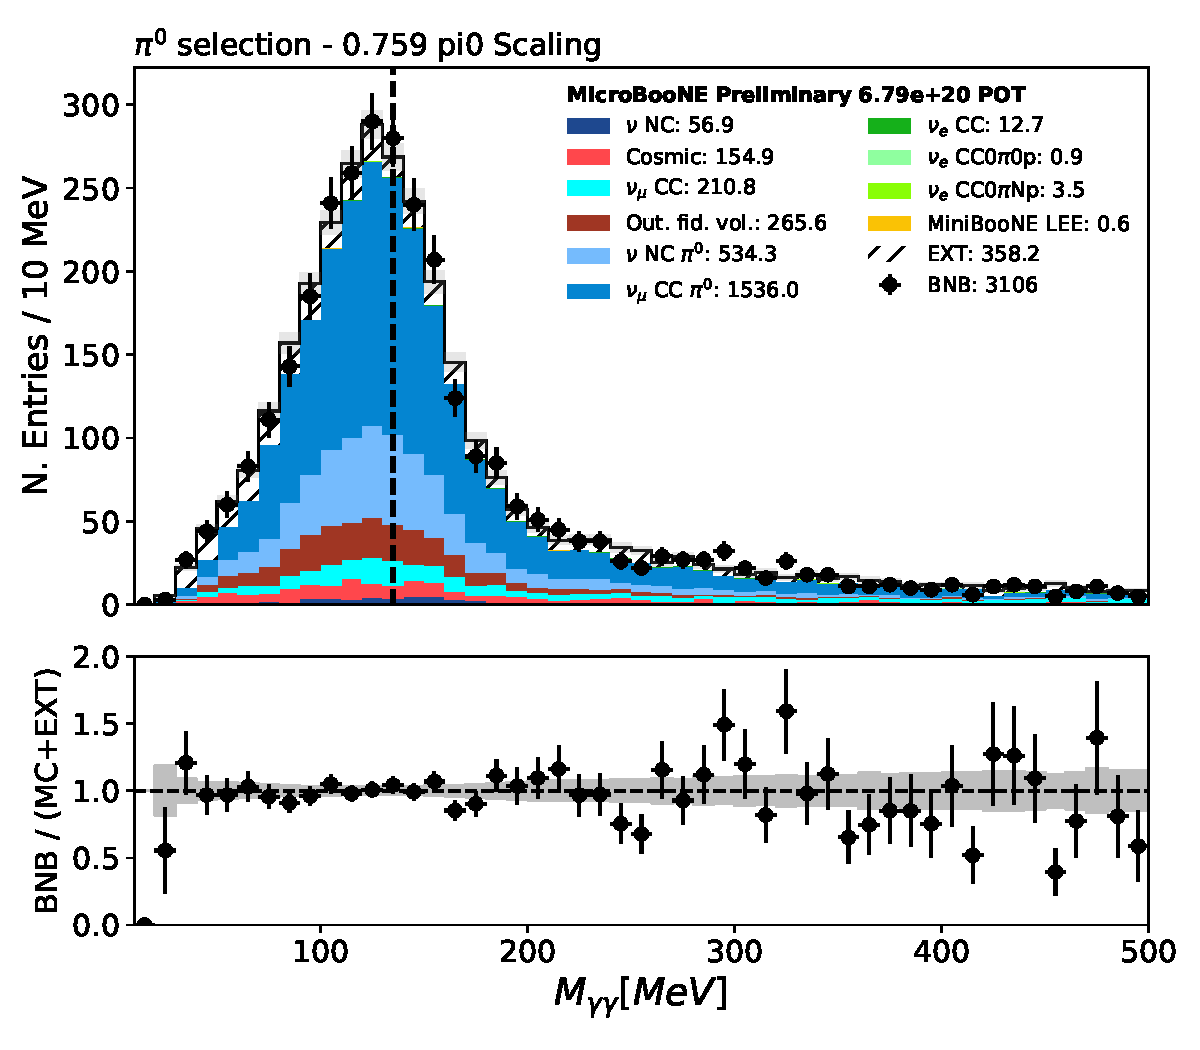
\includegraphics[width=0.65\textwidth]{pi0/calorimetry/pi0_mass_Y_corr_run123.pdf}
\caption{\label{fig:pi0massscaled}Reconstructed $\pi^0$ mass after a scaling of the $\pi^0$ production rate by 0.76. The energy scale of data and MC is calibrated and corrected by the same energy bias factor of $0.83$ computed for electrons in Sec.~\ref{sec:ereco}. While the correction applied is derived from electron showers in MC, it leads to a peak of the $M_{\gamma\gamma}$ distribution well aligned with the expected $\pi^0$ mass of 135 MeV, denoted by the dotted vertical line. This provides a strong validation of the energy-scale calibrations performed for EM showers in the $\nu_e$ analysis.}
% 07/24 p-value 0.3115 chisq/dof = 52.27/48
\end{center}
\end{figure}


\begin{figure}[H] 
\begin{center}
    \begin{subfigure}[b]{0.4\textwidth}
    \centering
    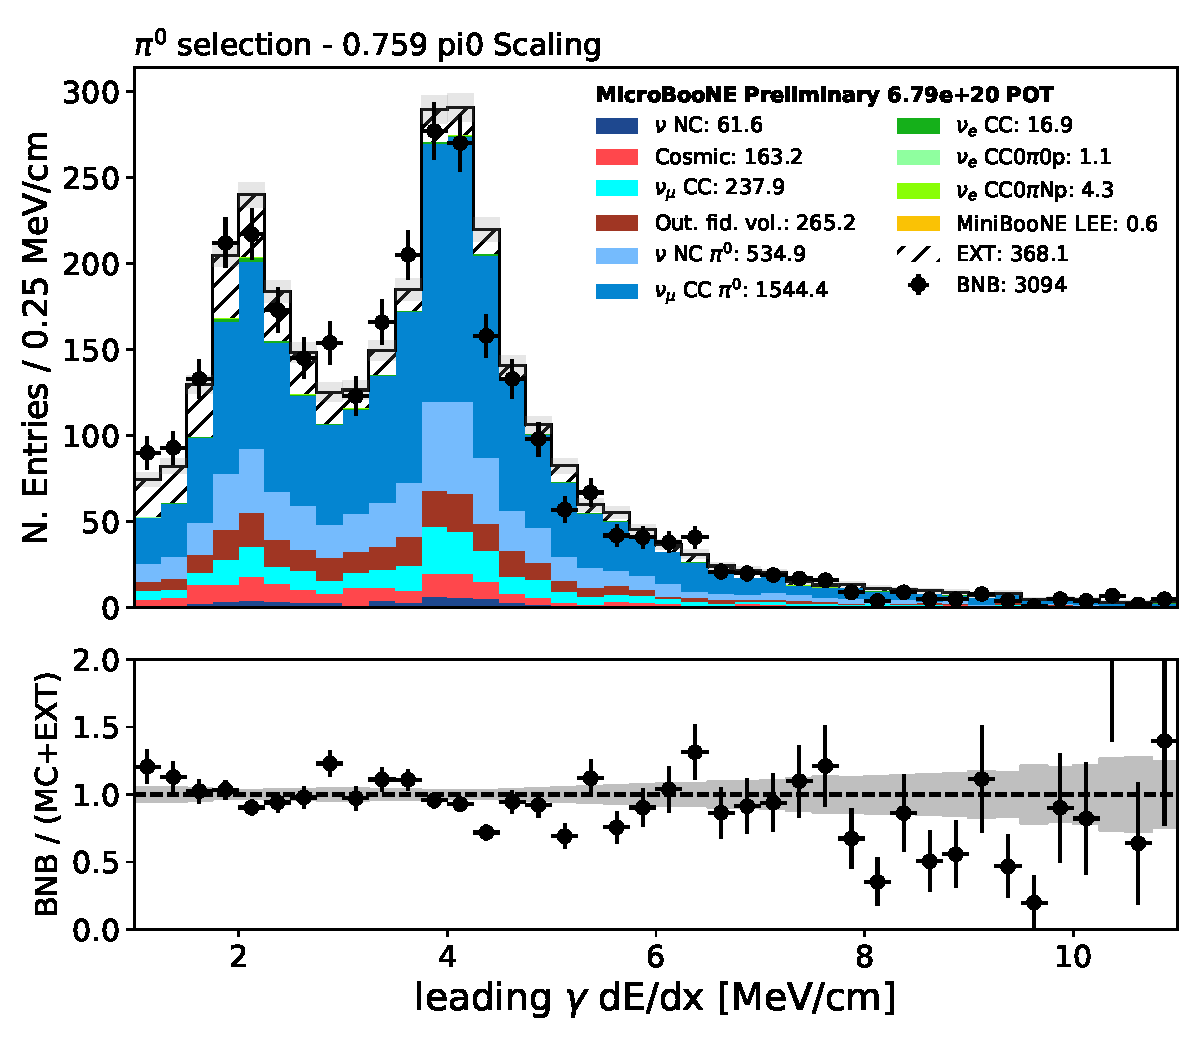
\includegraphics[width=1.00\textwidth]{pi0/calorimetry/pi0_dedx1_fit_Ypi0_dedx1_fit_Y_run123.pdf}
    \caption{all showers}
    \end{subfigure}
    \begin{subfigure}[b]{0.4\textwidth}
    \centering
    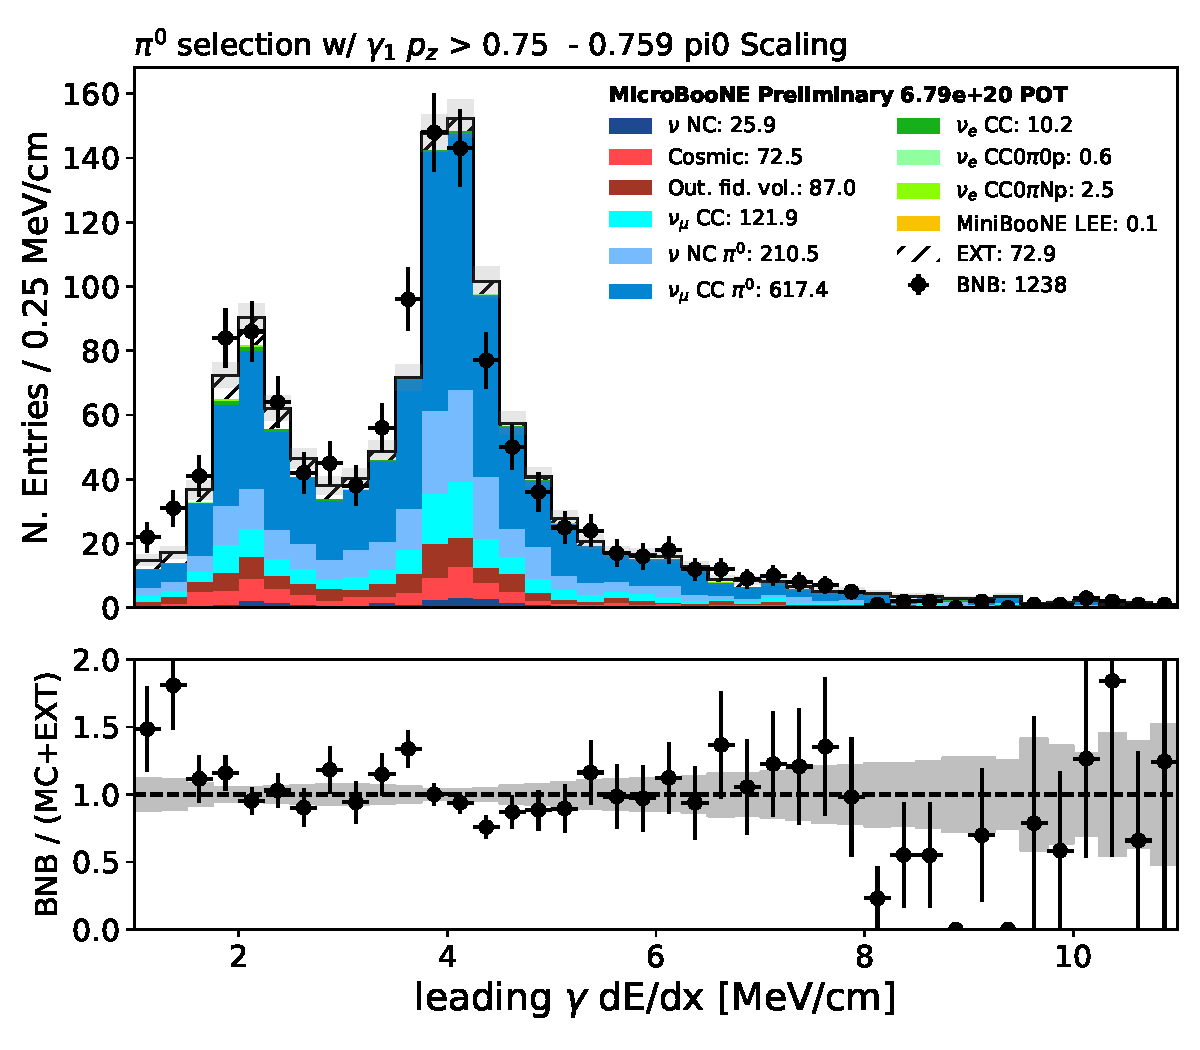
\includegraphics[width=1.00\textwidth]{pi0/calorimetry/pi0_dedx1_fit_Ypi0_dedx1_fit_Y_pz075_run123.pdf}
    \caption{shower $P_z > 0.75$}
    \end{subfigure}
    
\caption{Reconstructed \dedx calculated in the first 4 cm on the collection plane. The left image shows a comparison of data and simulation for all leading showers. The right image focuses on those showers with a $z$ component of momentum $>$ 0.75. The approximately one-bin offset in data relative to MC is due to detector mismodeling of the reconstructed charge and will be discussed more in section~\ref{sec:systematics}.}
\label{fig:pi0:dedxbest}
\end{center}
\end{figure}

\subsubsection{$\pi^0$ modeling}
\label{sec:pi0tune}
\par Measurements of MicroBooNE data rich in $\pi^0$ events have shown significant tension with MC expectations. The observations made from these datasets show an indication of an energy-dependent mis-modeling, with better data/mc agreement at lower $\pi^0$ (or total neutrino) energy and a stronger deficit in data at higher values. Based on these observations, a $\pi^0$-tune was developed with the aim of:
\begin{enumerate}
    \item Performing a data-driven constraint of $\pi^0$ events in MicroBooNE data as a function of $\pi^0$ energy and motivated by the energy-dependent data/mc discrepancies observed.
    \item Validate that the tune we obtain shows good data/MC agreement in $\pi^0$ rich sidebands across all variables, and in particular for selections that are very close to the $\nu_e$ signal region.
    \item Study the impact of the obtained tune on the predicted $\pi^0$ backgrounds to the eLEE analysis.
\end{enumerate}
The tune is performed by fitting for the contribution of $\pi^0$ events in our MC in the 2+ shower sideband (rich in $\pi^0$s and sharing the $\nu_e$ pre-selection as the electron analysis) in the distribution of reconstructed $\pi^0$ energy. The fit is performed by applying an energy-dependent weight to the true $\pi^0$ energy. The weight is defined as:
\begin{equation}
  \text{weight}=\left\{
  \begin{array}{@{}ll@{}}
    1 - w \times E_{\pi} [\text{GeV}], & \text{if}\ E_{\pi} < 0.6 \text{GeV} \\
    1 - w \times 0.6, & \text{otherwise}
  \end{array}\right.
\end{equation} 
The fit in a distribution of reconstructed energy is motivated by the good energy resolution obtained for $\pi^0$s, shown in figure~\ref{fig:pi0eres}. The result of the fit scanning the parameter $w$ is shown in figure~\ref{fig:pi0fitresult}, indicating a fit value of $0.4$. The reconstructed $\pi^0$ energy spectrum after the fit is shown in figure~\ref{fig:pi0fitspectrum}, with good normalization and shape agreement.


%\begin{comment}
\begin{figure}[H] 
\begin{center}
    \begin{subfigure}[b]{0.3\textwidth}
    \centering
    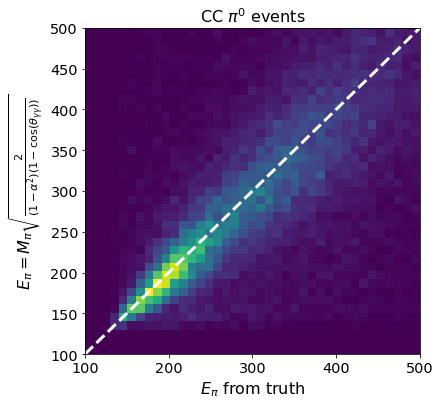
\includegraphics[width=1.00\textwidth]{pi0/pi0tune/ccpi0.png}
    \caption{\label{fig:pi0eres} $\pi^0$ energy resolution.}
    \end{subfigure}
    \begin{subfigure}[b]{0.27\textwidth}
    \centering
    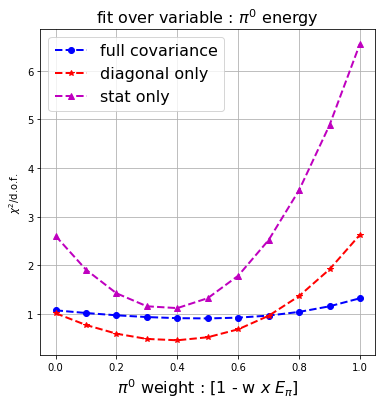
\includegraphics[width=1.00\textwidth]{pi0/pi0tune/chisq_pi0energy.png}
    \caption{\label{fig:pi0fitresult} $\pi^0$ fit result.}
    \end{subfigure}
    \begin{subfigure}[b]{0.33\textwidth}
    \centering
    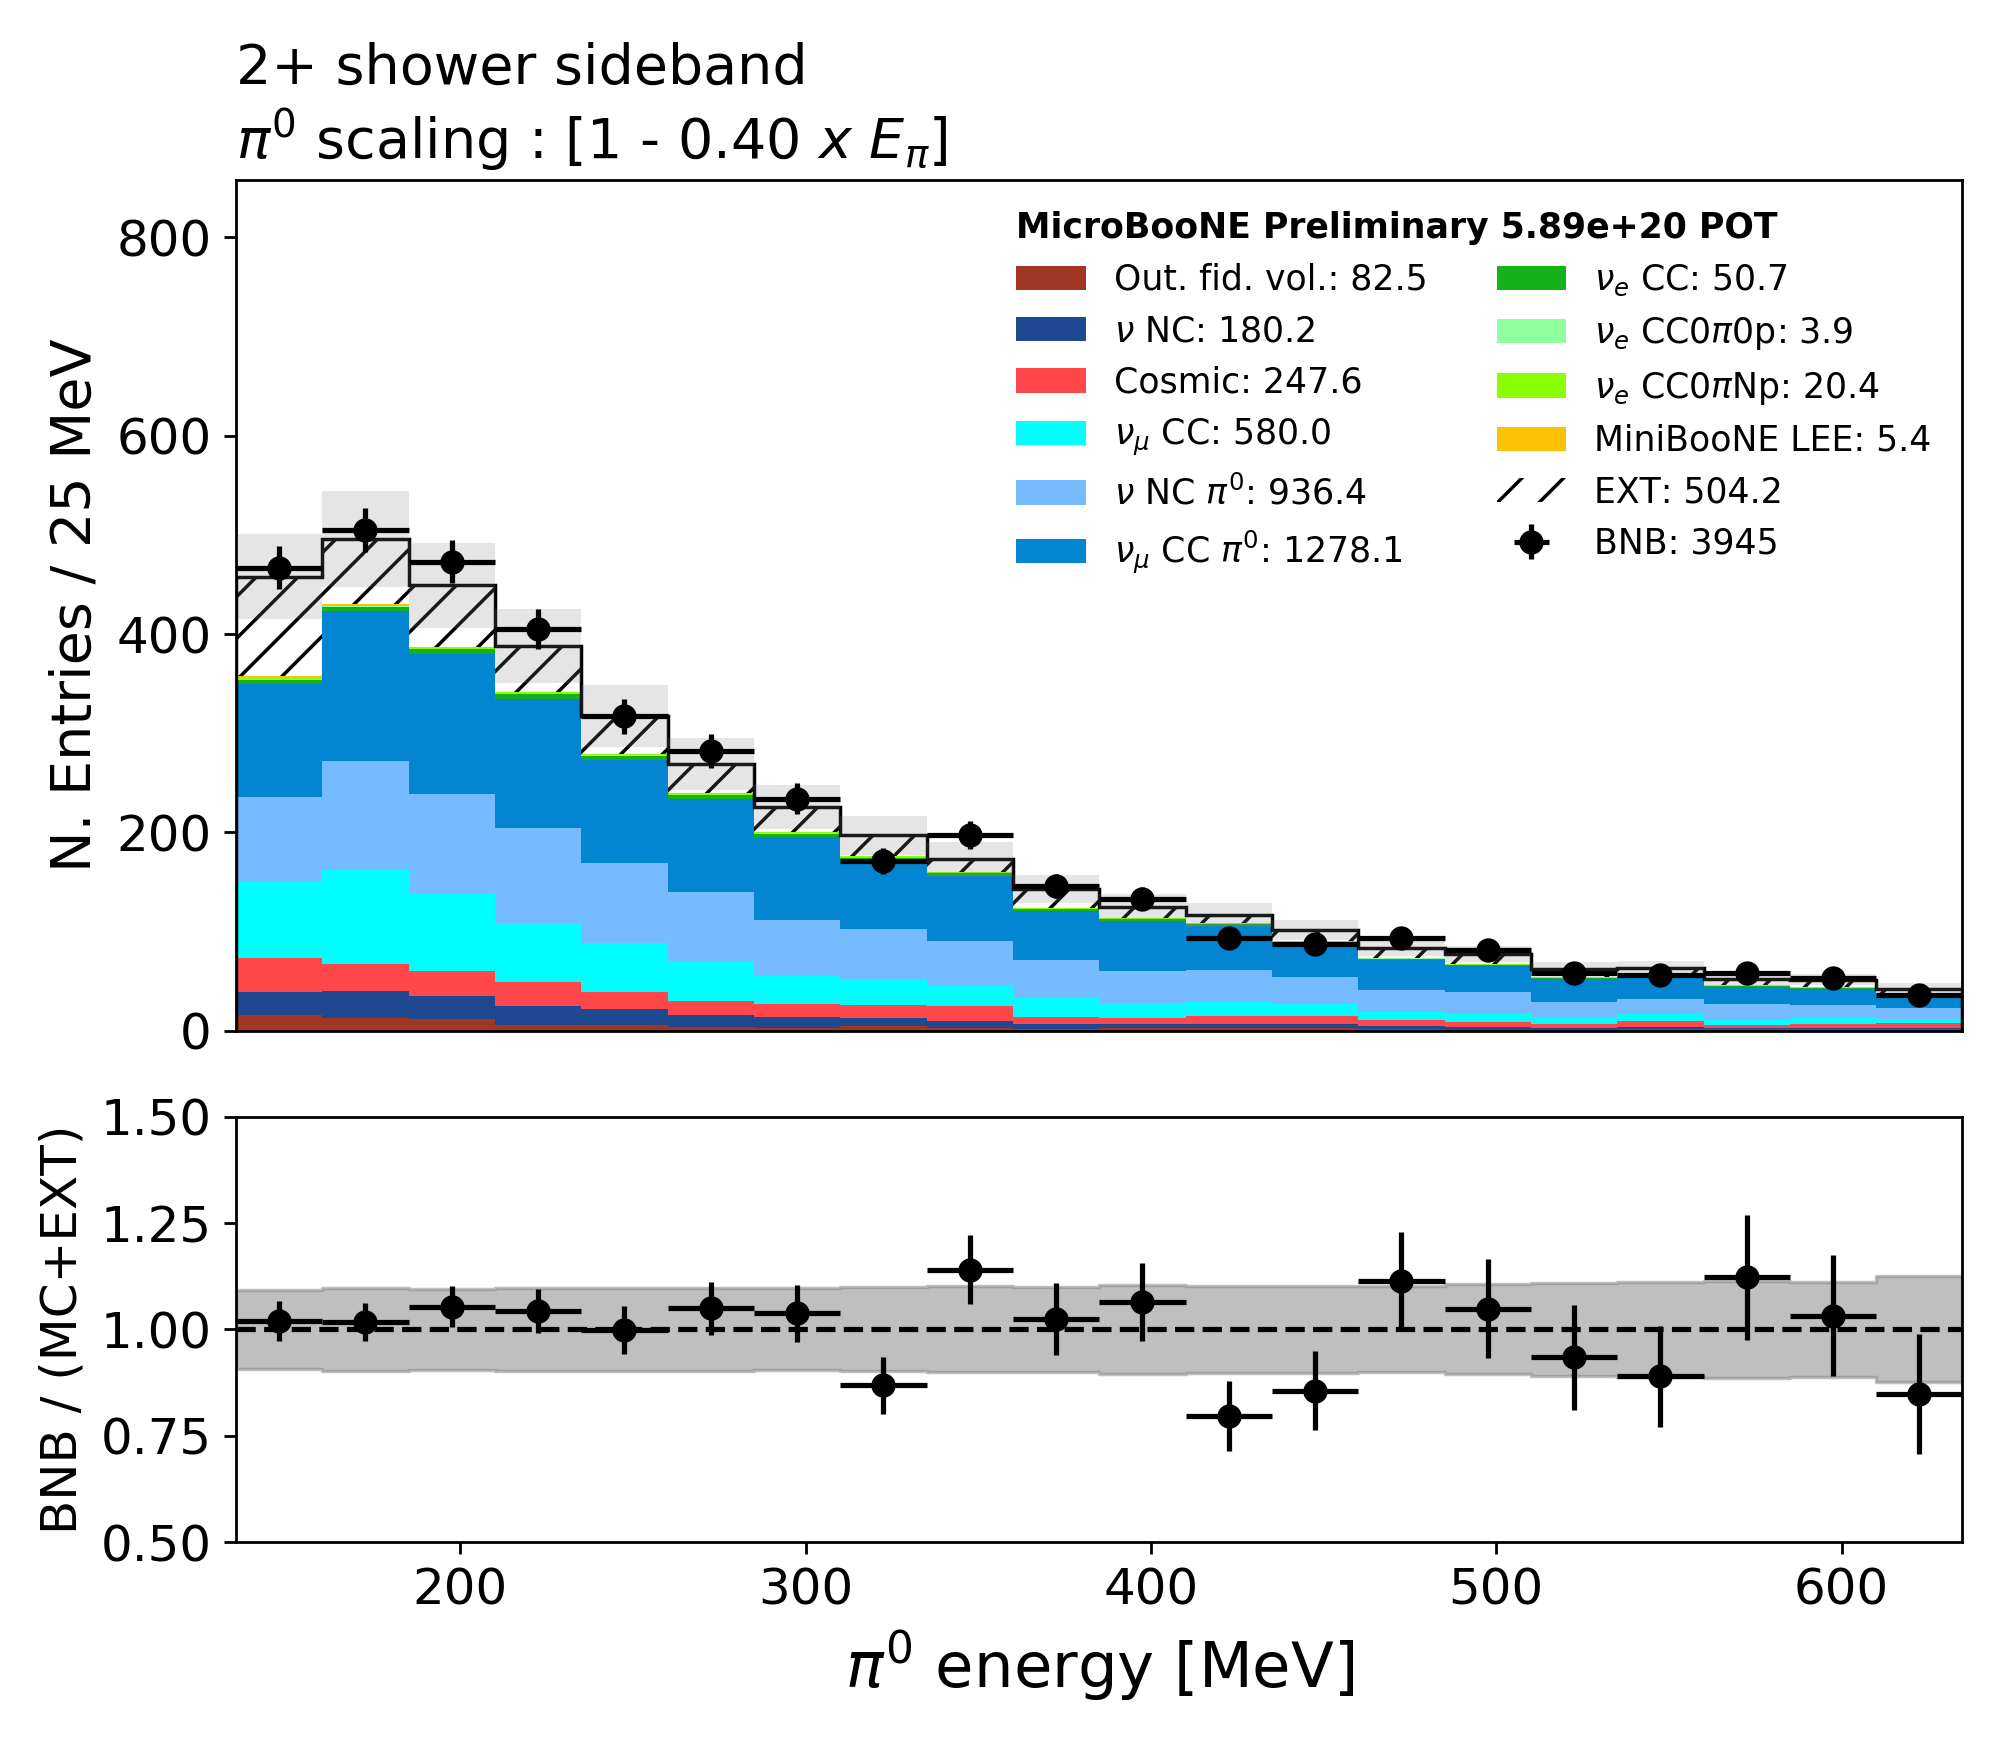
\includegraphics[width=1.00\textwidth]{pi0/pi0tune/pi0energy_040_scaling.png}
    \caption{\label{fig:pi0fitspectrum}energy spectrum post fit.}
    \end{subfigure}
%\caption{\label{fig:pi0fit}Various sidebands rich in $\pi^0$ events with default CV weights (left) and after applying the $\pi^0$ energy-dependent weight obtained from the 2+ shower sideband fit to data (middle spectrum). The consistently improved data/MC agreement across our siebands gives confidence in the robustness of this tune and its ability to correctly model $\pi^0$ backgrounds for the eLEE analysis.}
\end{center}
\end{figure}

The validity of the tune is checked by performing the same fit procedure over multiple variables in the same sideband. These cross-check are found to give a consistent best fit at $w = 0.4$. Additionally, we test the tune by comparing data/MC agreement before and after the tune is implemented on three different sidebands: the $\pi^0$ sideband (figures~\cref{fig:pi0tune00,fig:pi0tune01}), 2+ shower sideband (figures~\cref{fig:pi0tune02,fig:pi0tune03}), and one-shower sideband (figures~\cref{fig:pi0tune04,fig:pi0tune05}). All show an improvement in data/mc agreement when comparing pre-tune (left) and post-tune (right) distributions. The absolute data/mc agreement after the tune is within systematics for all three sidebands.

%\end{comment}


\begin{figure}[H] 
\begin{center}
    \begin{subfigure}[b]{0.45\textwidth}
    \centering
    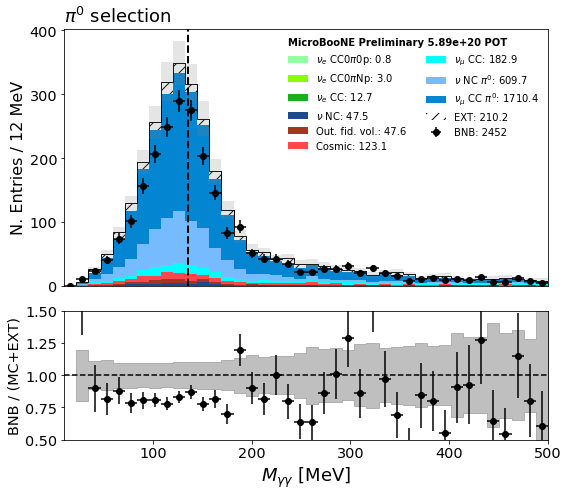
\includegraphics[width=1.00\textwidth]{pi0/pi0tune/mass_noscaling.png}
    \caption{\label{fig:pi0tune00} $\pi^0$ sideband pre-tune.}
    \end{subfigure}
    \begin{subfigure}[b]{0.45\textwidth}
    \centering
    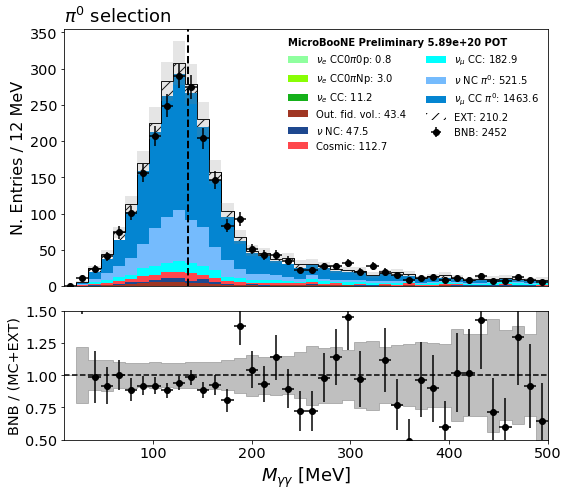
\includegraphics[width=1.00\textwidth]{pi0/pi0tune/mass_energycaling.png}
    \caption{\label{fig:pi0tune01} $\pi^0$ sideband post-tune.}
    \end{subfigure}
    \begin{subfigure}[b]{0.45\textwidth}
    \centering
    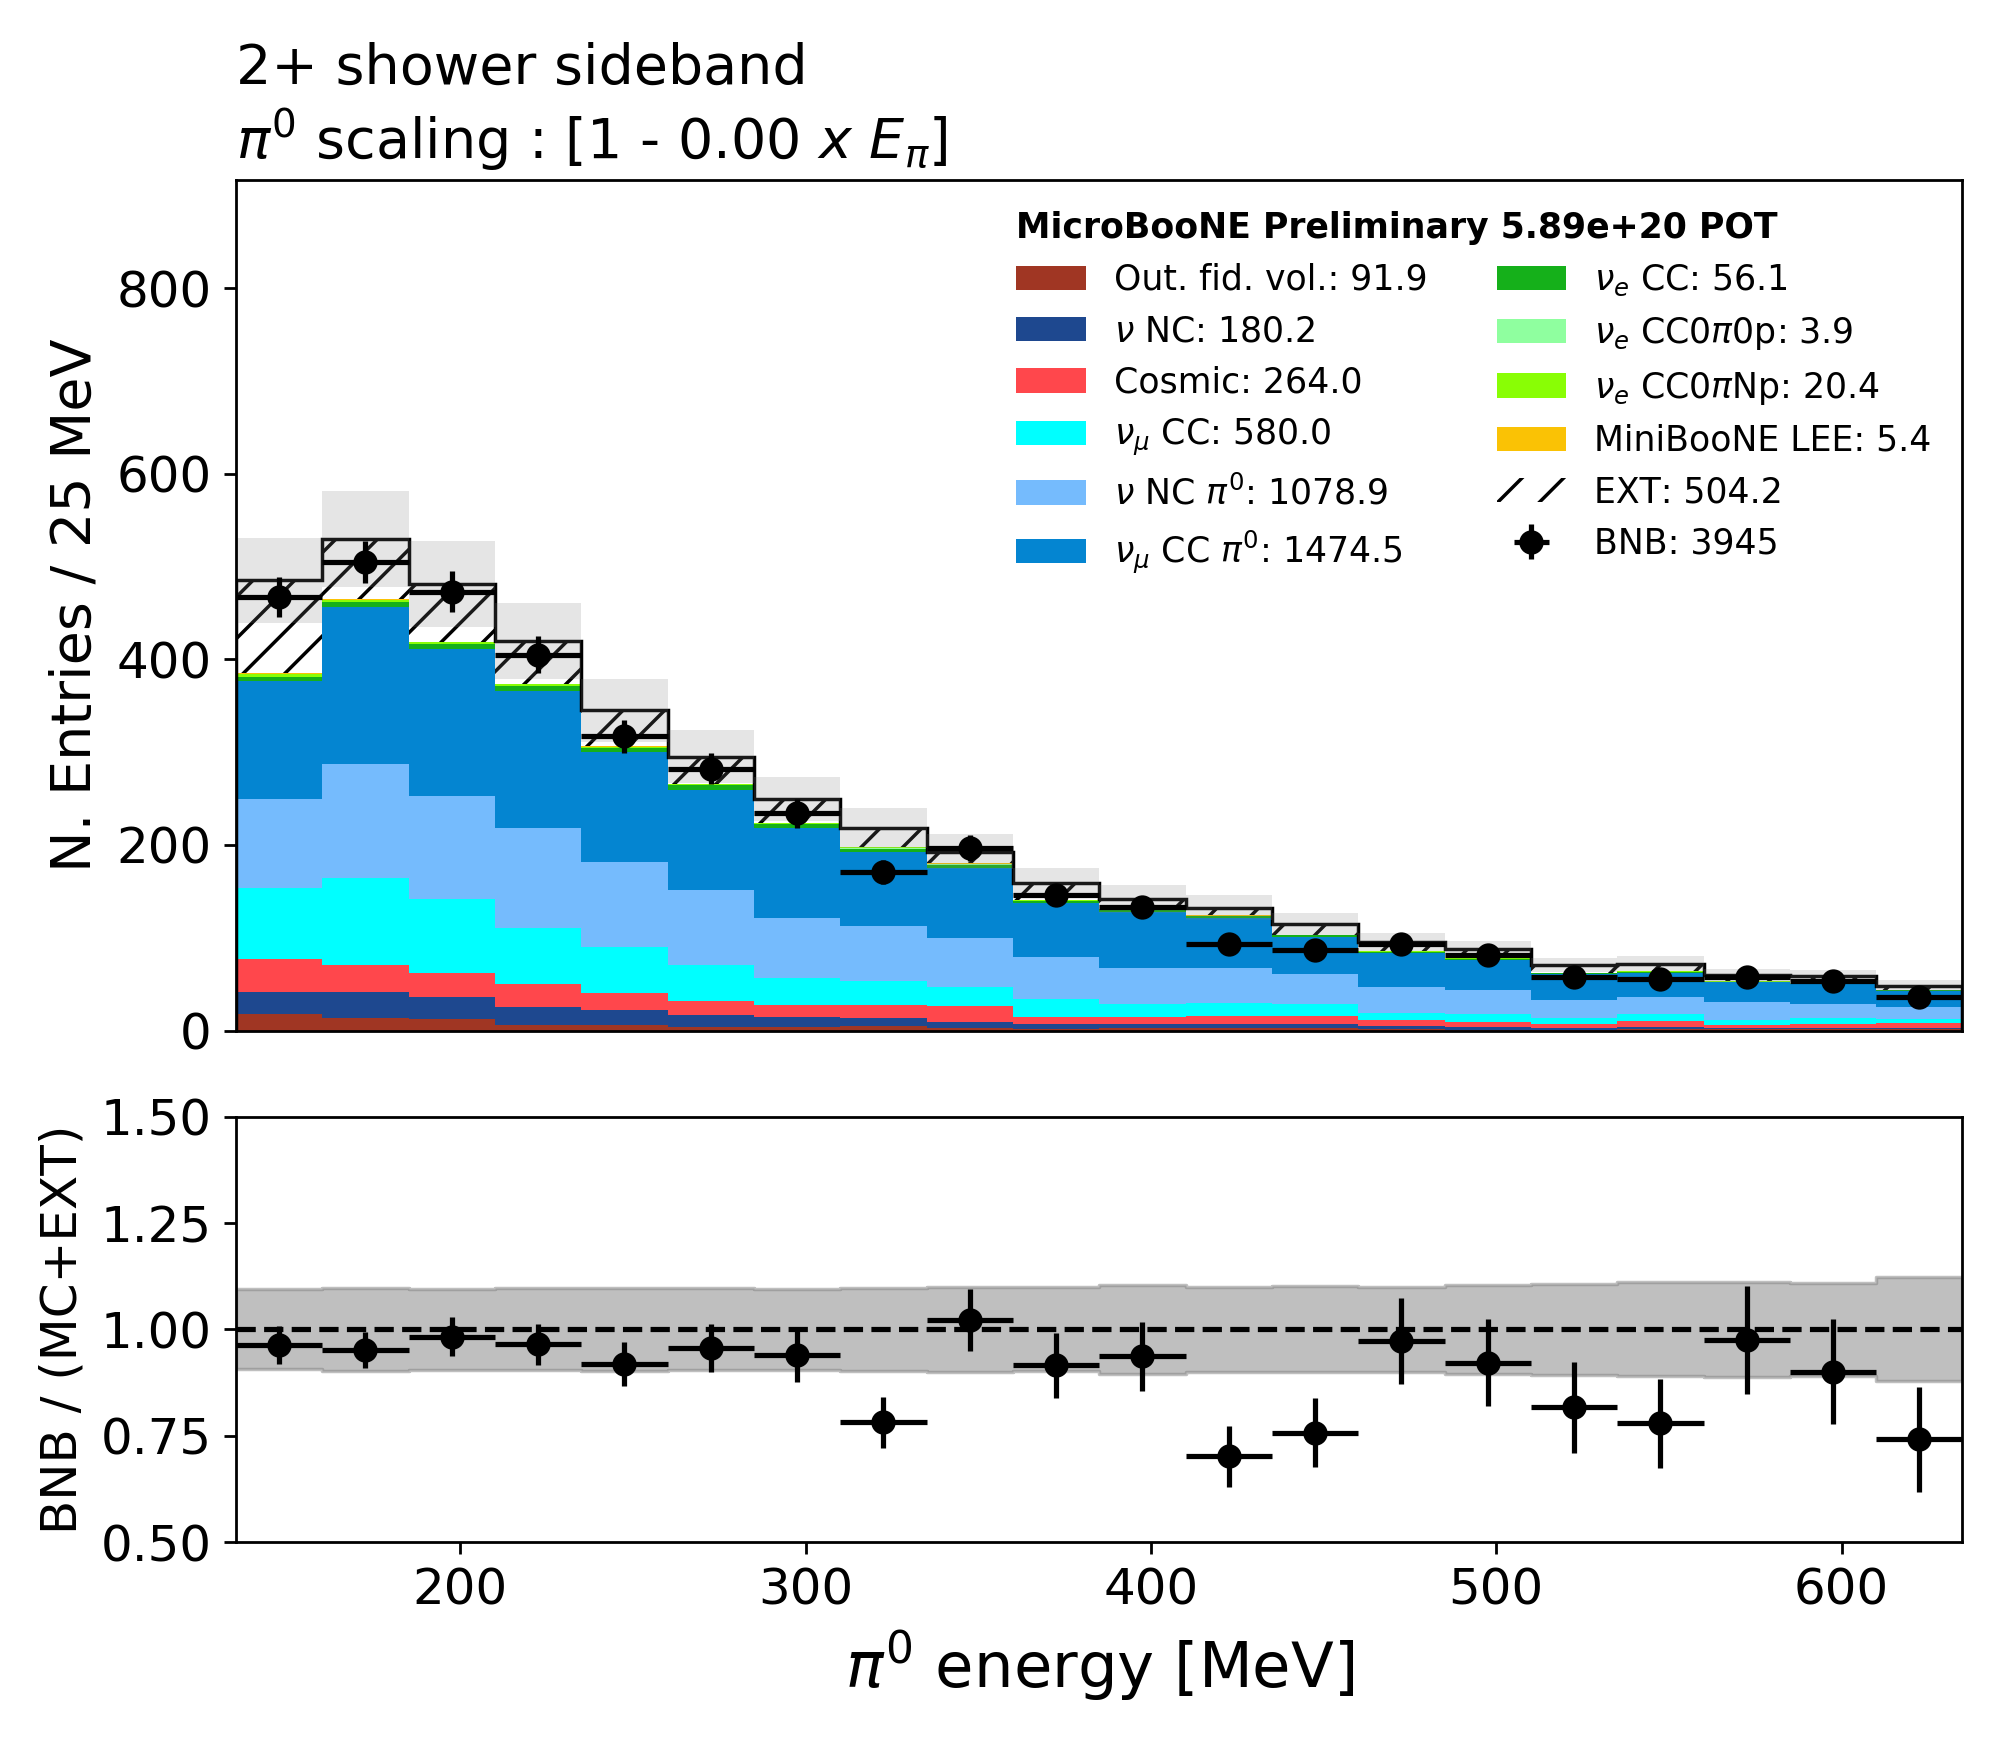
\includegraphics[width=1.00\textwidth]{pi0/pi0tune/pi0energy_000_scaling.png}
    \caption{\label{fig:pi0tune02} 2+ shower sideband pre-tune.}
    \end{subfigure}
    \begin{subfigure}[b]{0.45\textwidth}
    \centering
    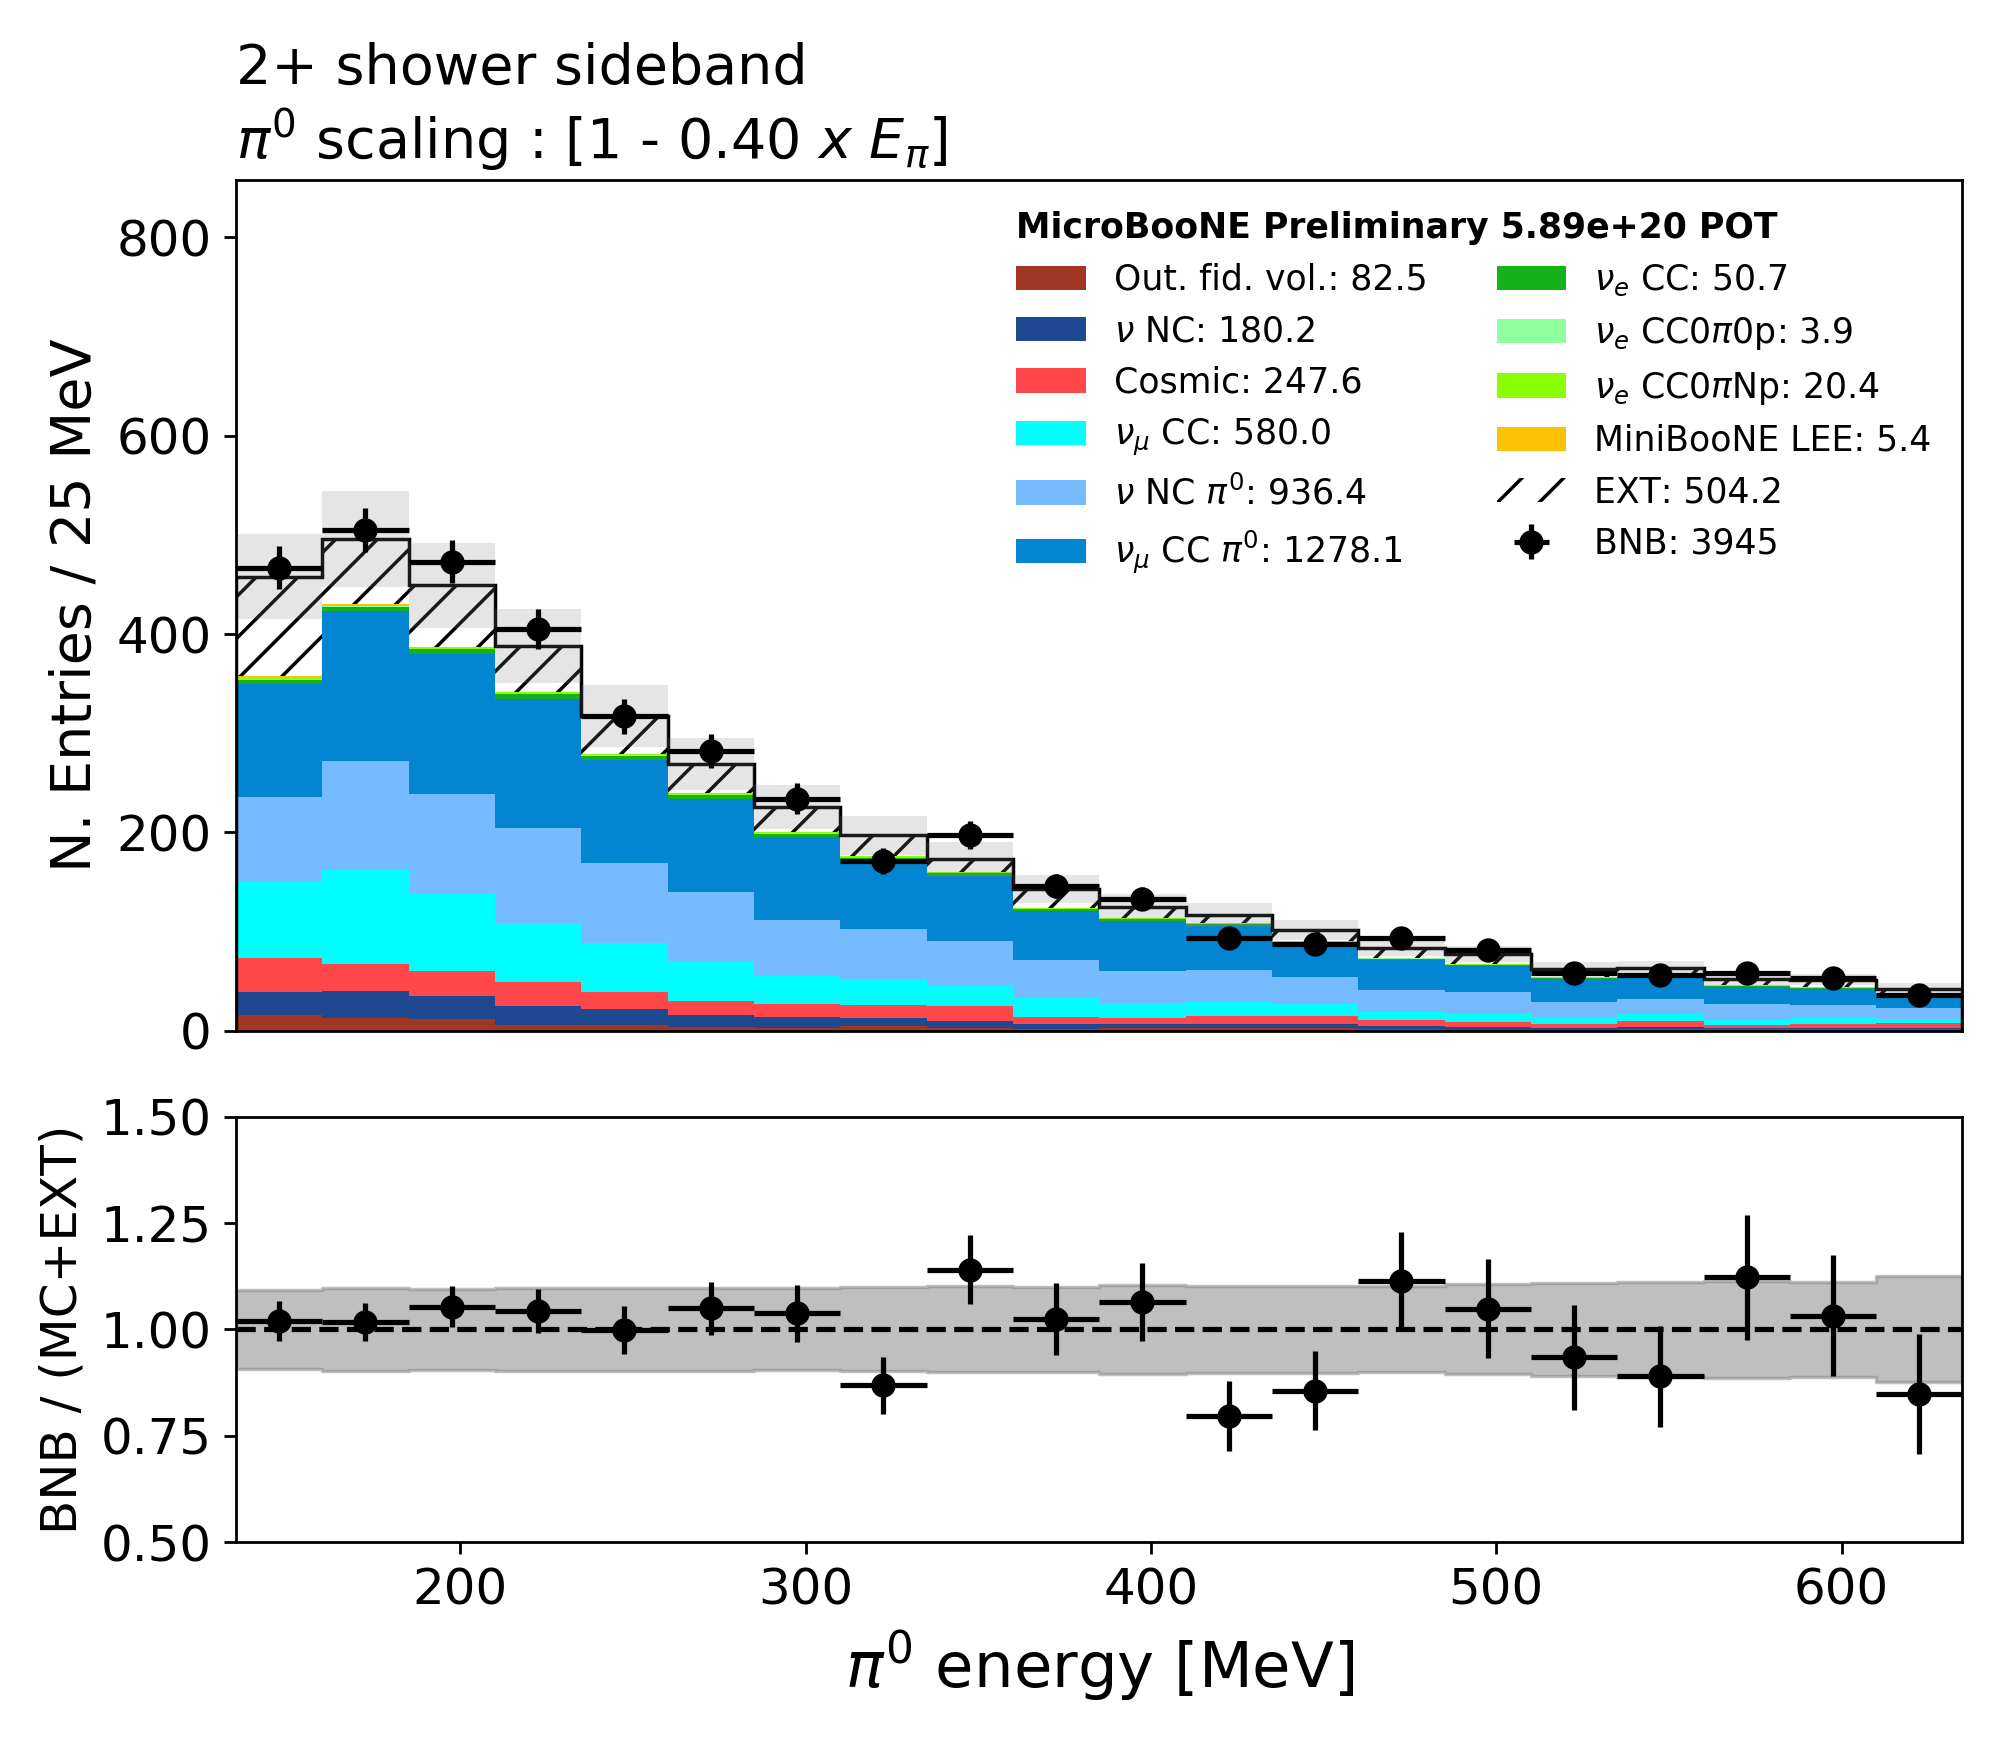
\includegraphics[width=1.00\textwidth]{pi0/pi0tune/pi0energy_040_scaling.png}
    \caption{\label{fig:pi0tune03} 2+ shower sideband post-tune.}
    \end{subfigure}
    \begin{subfigure}[b]{0.45\textwidth}
    \centering
    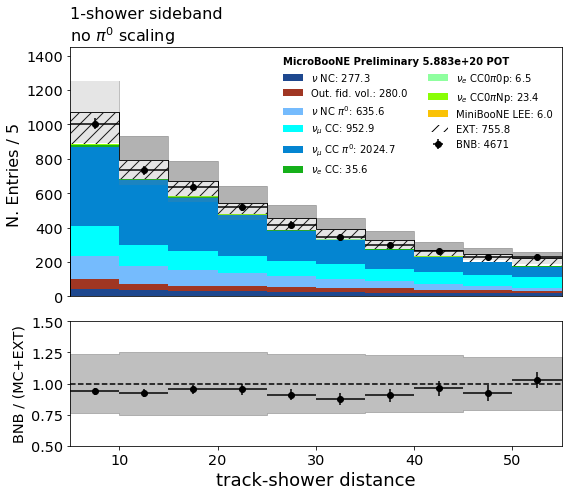
\includegraphics[width=1.00\textwidth]{pi0/pi0tune/tksh_distance_1shr_noscaling.png}
    \caption{\label{fig:pi0tune04} 1 shower sideband pre-tune.}
    \end{subfigure}
    \begin{subfigure}[b]{0.45\textwidth}
    \centering
    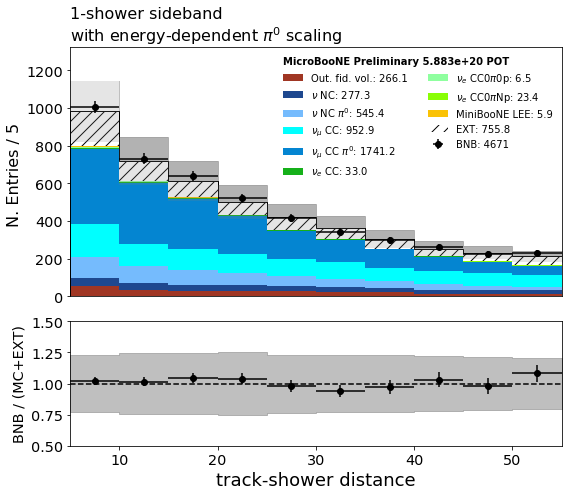
\includegraphics[width=1.00\textwidth]{pi0/pi0tune/tksh_distance_1shr.png}
    \caption{\label{fig:pi0tune05} 1 shower sideband post-tune.}
    \end{subfigure}
\caption{\label{fig:pi0norm}Various sidebands rich in $\pi^0$ events with default CV weights (left) and after applying the $\pi^0$ energy-dependent weight obtained from the 2+ shower sideband fit to data (middle spectrum). The consistently improved data/MC agreement across our siebands gives confidence in the robustness of this tune and its ability to correctly model $\pi^0$ backgrounds for the eLEE analysis.}
\end{center}
\end{figure}

\subsection{Stopping muons and protons}
\label{sec:sideband:stopping_muons_protons}

In order to study in detail the reconstruction of the calorimetry, with specific attention to the accuracy of the simulation, detailed high-statistic and fine-binned data/simulation comparisons have been performed.
Data/simulation comparsions of muon or proton \dedx are impacted by the underlying angular and energy distributions of protons produced in neutrino interactions, an aspect of $\nu$-Ar modeling particularly prone to modeling uncertainties in the case of protons. Discrepancies due to the detector mis-modelling of \dedx cannot therefore disentangled from mis-modelling of the underlying kinematic distributions.
Because of this, we realised the importance of comparing distributions of \dqdx or \dedx in fine bins of relevant variables such as residual range (a proxy for energy) and angle to disentangle cross-section from detector effects.

All the validation plots shown in this section are performed by comparing the \dqdx distribution from the data with the simulation.
The plots are filled once per hit, and they are area normalised as after subtracting beam-OFF contributions.% are subtracted from beam ON events after being normalized to the the number of triggers.
%As a second step, the simulation is weighted with the latest GENIE weights, and then area normalised to the data beam ON - beam OFF.

The main purpose of this study is to validate the simulation after applying the re-calibration and test the impact of recombination.
Here we report a subset of the studies that have been performed, concluding from them that the re-calibration employed recovers the bulk of data-mc differences observed and allows to make strong use of calorimetric information for PID in the analysis in a robust way.
The interested reader can find a complete list of plots of data/simulation comparison in \cite{bib:pid_internal_note}.

\paragraph{Stopping muons}
A purely geometrical selection (i.e. without using any calorimetric information) of neutrino-induced stopping muons has been performed, achieving a purity of neutrino-induced muons of about 57\%, that becomes 73\% when we subtract the Beam OFF data.
This allows testing the effect of the re-calibration, by looking at the MIP-like region of stopping muons, considering only hits at residual range $>$ 30 cm.
This region should show similar data/simulation discrepancies to what was observed with the ACPTs.
Figure \ref{fig:stopping_muons_large_rr_high_pitch} shows the data/simulation comparisons of the \dqdx distribution before (left) and after (right) re-calibration, in a bin of high pitch and $\phi$, where re-calibration corrections are larger.
We notice considerable improvement of the accuracy of the simulation, although it does not fully recover data/MC differences.
%It is noteworthy that the corrections needed in the two angular bins are significantly different, even visually.
%This reinforces again the importance of correcting the simulation as a function of the angular variables.

\begin{figure}[H] 
\begin{center}
    \begin{subfigure}[b]{0.45\textwidth}
    \centering
    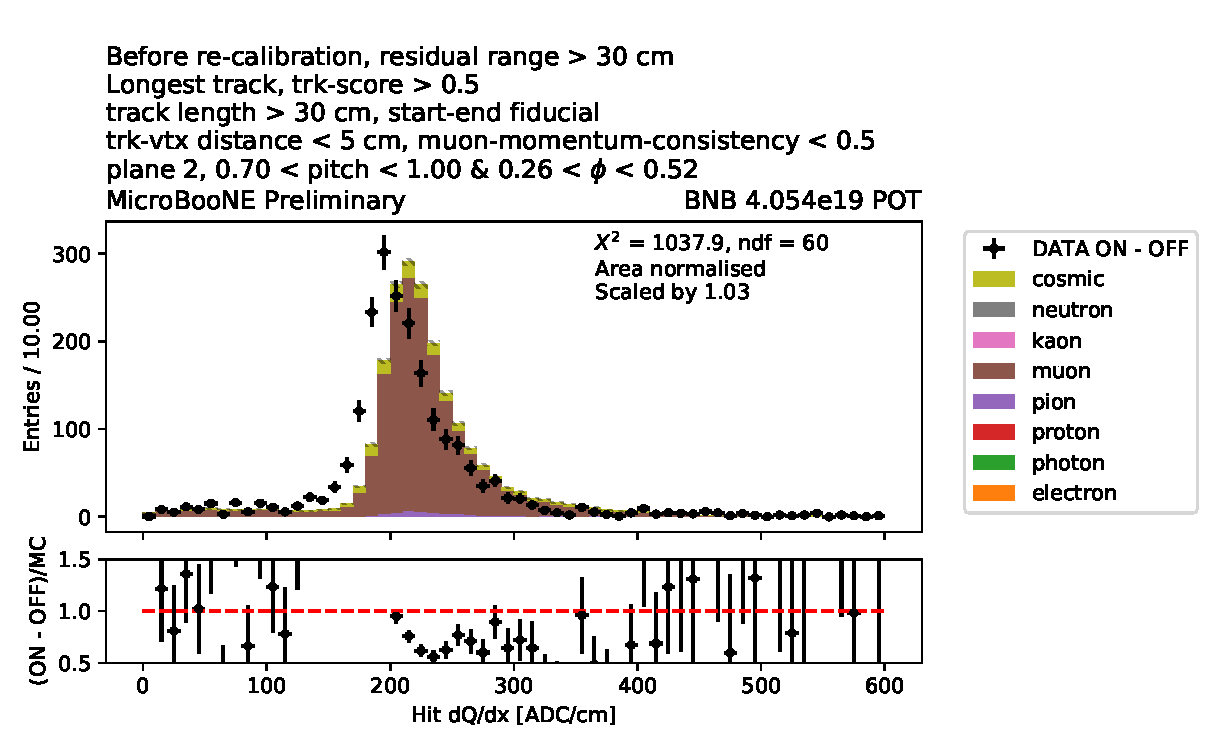
\includegraphics[width=1.00\textwidth]{stopping_muons_protons/070_pitch_100_026_phi_052apres.pdf}
    \end{subfigure}
    \begin{subfigure}[b]{0.45\textwidth}
    \centering
    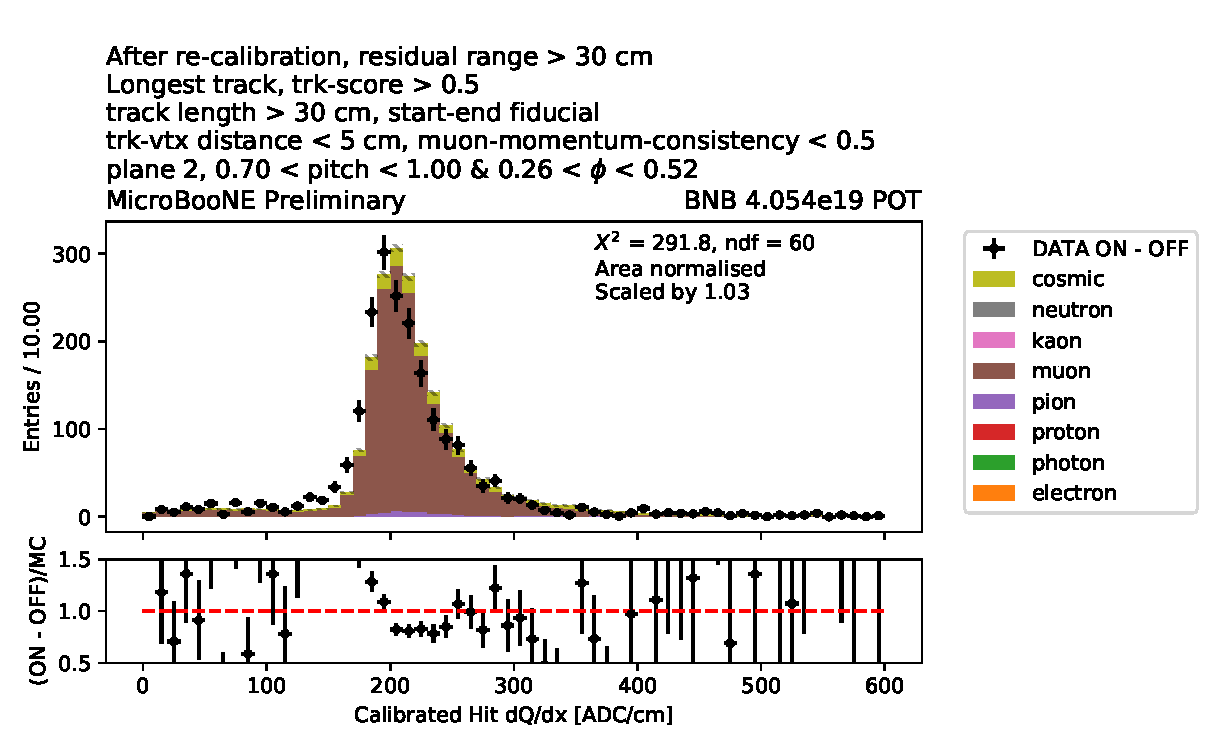
\includegraphics[width=1.00\textwidth]{stopping_muons_protons/070_pitch_100_026_phi_052depois.pdf}
    \end{subfigure}
\caption{Data/simulation comparison of the \dqdx distributions before (left) and after (right) the re-calibration, for stopping muons in the MIP-like region, with residual range $>$ 30 cm, and the bin with 0.7 cm $<$ pitch $<$ 1 cm.}
\label{fig:stopping_muons_large_rr_high_pitch}
\end{center}
\end{figure}

\paragraph{Stopping protons and the effect of recombination}
In order to study how well the effect of recombination is simulated, it is very useful to look at protons at very small residual range, where the ionisation density is very large and the non-linear \dedx $\rightarrow$ \dqdx response becomes apparent.
A proton selection based on both geometrical cuts and a cut on the PID score has been designed for this purpose, achieving a purity of neutrino-induced protons of about 78\%, that becomes 85\% when we subtract the Beam OFF data.
In order to disentangle recombination from detector effects, the following plots are restricted to the region at small pitch, between 0.3 and 0.4 cm.
The two plots shown in Figures \ref{fig:stopping_protons_recombination} show the comparisons, after the re-calibration, for stopping protons with residual range between 5 and 10 cm, and 10 and 20 cm, respectively.

\begin{figure}[H] 
\begin{center}
    \begin{subfigure}[b]{0.45\textwidth}
    \centering
    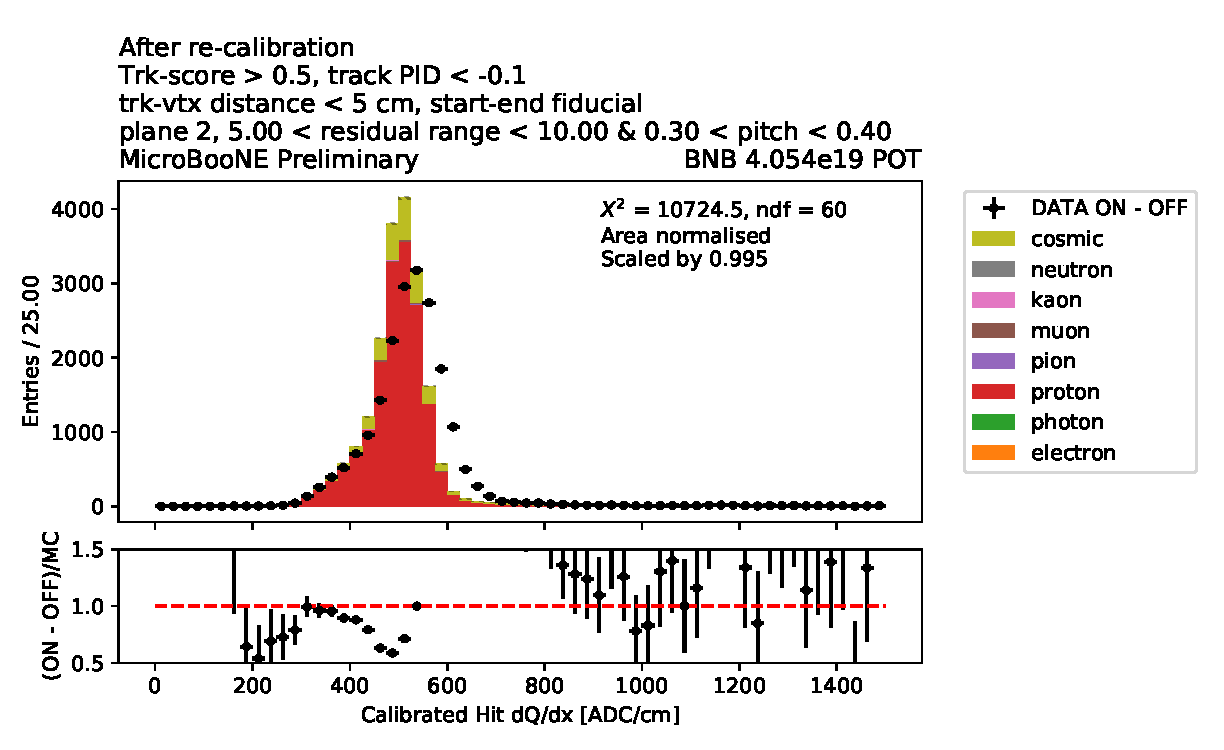
\includegraphics[width=1.00\textwidth]{stopping_muons_protons/protons_500_residualrange_1000_030_pitch_040depois.pdf}
    \end{subfigure}
    \begin{subfigure}[b]{0.45\textwidth}
    \centering
    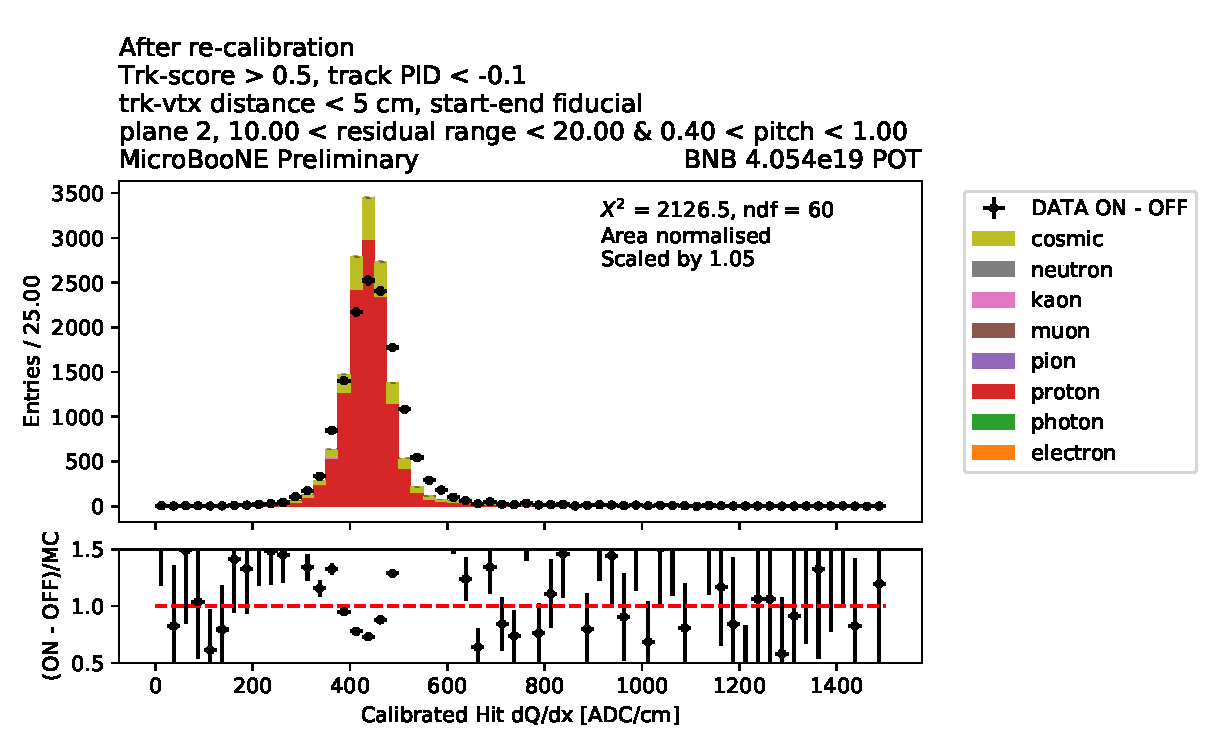
\includegraphics[width=1.00\textwidth]{stopping_muons_protons/protons_1000_residual_range_2000_040_pitch_100depois.pdf}
    \end{subfigure}
\caption{Data/simulation comparison of \dqdx after the re-calibration, for stopping protons with 0.3 cm $<$ pitch $<$ 0.4 cm and 5 cm $<$ residual range $<$ 19 cm (left plot), and 10 cm $<$ residual range $<$ 20 cm (right plot).}
\label{fig:stopping_protons_recombination}
\end{center}
\end{figure}
The overall agreement in the peaks of data and MC distributions suggest that no substantial non-linear effect in the calibration is present, and therefore the calorimetric information being used in the analysis is validaetd over a broad range of \dedx covering MIP muons to highly ionizing low-energy protons.
This is also confirmed also by the good agreement between the data and the theory seen in Figure \ref{fig:llr_pid_pdf_example}.

%We believe the simulation, although not perfect, reproduces all features observed in the data, and it is thus good enough for the rest of the analysis.

The studies shown in this section after the re-calibration, while showing residual data/simulation discrepancies limited to specific regions of the phase space, give us confidence in having reached a level of detector modeling adequate for the successful performance of this analysis. 
The impact of detector mis-modeling is further evaluated in terms of the systematic impact of detector effects in \ref{sec:detsys}.

\paragraph{Limitations}
Despite the good degree of accuracy, we realise that the current calorimetric reconstruction and the methods developed in this analysis contain several limitations.

As previously observed, in certain bins the re-calibration only corrects the scale of the distribution, lacking of an additional smearing which leads to shape disagreement in the width of \dedx distributions.
Additionally, the re-calibration applied to neutrino-induced particles is in general not as effective as on the ACPTs.
We have seen that the scale of the distribution is still not accurate even after the re-calibration, and in certain bins, the correction even goes in the opposite direction with respect to the discrepancy.
We understood these effects are related, at least partially, to the coarseness of the bins in which the re-calibration is computed.
With coarse bins, the difference between ACPTs and neutrino-induced particles in the angular distributions in every single bin become relevant, producing calibration factors which are not very accurate for the neutrino induced particles.

All these studies have been documented in detail in \cite{bib:pid_internal_note}, which contains all data/simulation comparisons in all bins of phase space.

